% Options for packages loaded elsewhere
\PassOptionsToPackage{unicode}{hyperref}
\PassOptionsToPackage{hyphens}{url}
%
\documentclass[
]{article}
\usepackage{amsmath,amssymb}
\usepackage{iftex}
\ifPDFTeX
  \usepackage[T1]{fontenc}
  \usepackage[utf8]{inputenc}
  \usepackage{textcomp} % provide euro and other symbols
\else % if luatex or xetex
  \usepackage{unicode-math} % this also loads fontspec
  \defaultfontfeatures{Scale=MatchLowercase}
  \defaultfontfeatures[\rmfamily]{Ligatures=TeX,Scale=1}
\fi
\usepackage{lmodern}
\ifPDFTeX\else
  % xetex/luatex font selection
\fi
% Use upquote if available, for straight quotes in verbatim environments
\IfFileExists{upquote.sty}{\usepackage{upquote}}{}
\IfFileExists{microtype.sty}{% use microtype if available
  \usepackage[]{microtype}
  \UseMicrotypeSet[protrusion]{basicmath} % disable protrusion for tt fonts
}{}
\makeatletter
\@ifundefined{KOMAClassName}{% if non-KOMA class
  \IfFileExists{parskip.sty}{%
    \usepackage{parskip}
  }{% else
    \setlength{\parindent}{0pt}
    \setlength{\parskip}{6pt plus 2pt minus 1pt}}
}{% if KOMA class
  \KOMAoptions{parskip=half}}
\makeatother
\usepackage{xcolor}
\usepackage[margin=1in]{geometry}
\usepackage{longtable,booktabs,array}
\usepackage{calc} % for calculating minipage widths
% Correct order of tables after \paragraph or \subparagraph
\usepackage{etoolbox}
\makeatletter
\patchcmd\longtable{\par}{\if@noskipsec\mbox{}\fi\par}{}{}
\makeatother
% Allow footnotes in longtable head/foot
\IfFileExists{footnotehyper.sty}{\usepackage{footnotehyper}}{\usepackage{footnote}}
\makesavenoteenv{longtable}
\usepackage{graphicx}
\makeatletter
\def\maxwidth{\ifdim\Gin@nat@width>\linewidth\linewidth\else\Gin@nat@width\fi}
\def\maxheight{\ifdim\Gin@nat@height>\textheight\textheight\else\Gin@nat@height\fi}
\makeatother
% Scale images if necessary, so that they will not overflow the page
% margins by default, and it is still possible to overwrite the defaults
% using explicit options in \includegraphics[width, height, ...]{}
\setkeys{Gin}{width=\maxwidth,height=\maxheight,keepaspectratio}
% Set default figure placement to htbp
\makeatletter
\def\fps@figure{htbp}
\makeatother
\setlength{\emergencystretch}{3em} % prevent overfull lines
\providecommand{\tightlist}{%
  \setlength{\itemsep}{0pt}\setlength{\parskip}{0pt}}
\setcounter{secnumdepth}{-\maxdimen} % remove section numbering
\newlength{\cslhangindent}
\setlength{\cslhangindent}{1.5em}
\newlength{\csllabelwidth}
\setlength{\csllabelwidth}{3em}
\newlength{\cslentryspacingunit} % times entry-spacing
\setlength{\cslentryspacingunit}{\parskip}
\newenvironment{CSLReferences}[2] % #1 hanging-ident, #2 entry spacing
 {% don't indent paragraphs
  \setlength{\parindent}{0pt}
  % turn on hanging indent if param 1 is 1
  \ifodd #1
  \let\oldpar\par
  \def\par{\hangindent=\cslhangindent\oldpar}
  \fi
  % set entry spacing
  \setlength{\parskip}{#2\cslentryspacingunit}
 }%
 {}
\usepackage{calc}
\newcommand{\CSLBlock}[1]{#1\hfill\break}
\newcommand{\CSLLeftMargin}[1]{\parbox[t]{\csllabelwidth}{#1}}
\newcommand{\CSLRightInline}[1]{\parbox[t]{\linewidth - \csllabelwidth}{#1}\break}
\newcommand{\CSLIndent}[1]{\hspace{\cslhangindent}#1}
\ifLuaTeX
  \usepackage{selnolig}  % disable illegal ligatures
\fi
\IfFileExists{bookmark.sty}{\usepackage{bookmark}}{\usepackage{hyperref}}
\IfFileExists{xurl.sty}{\usepackage{xurl}}{} % add URL line breaks if available
\urlstyle{same}
\hypersetup{
  pdftitle={PREE\_Assignment},
  pdfauthor={Andres Mancera Barreto},
  hidelinks,
  pdfcreator={LaTeX via pandoc}}

\title{PREE\_Assignment}
\author{Andres Mancera Barreto}
\date{2023-09-19}

\begin{document}
\maketitle

\hypertarget{title}{%
\subsection{Title}\label{title}}

\hypertarget{the-islanders-a-mock-analysis-on-penguin-distribution-in-three-different-islands.}{%
\subsubsection{The islanders: a mock analysis on penguin distribution in
three different
islands.}\label{the-islanders-a-mock-analysis-on-penguin-distribution-in-three-different-islands.}}

\hypertarget{abstract}{%
\subsubsection{Abstract}\label{abstract}}

What can I say. There is available data of penguins in R that is not
mine but is free to use. There is an assignment about data
reproducibility that requires you to copy what I have done. This is me
trying to accomplish that and not destroy my chances of graduating in
the process. I hope it works.

\hypertarget{introduction}{%
\subsubsection{Introduction}\label{introduction}}

You know how introductions go. Start kind of broad on the topic, then
narrow down without pushing it too much. Insert claims from others that
help support your thesis (Carey \& Alexander, 2003; Cahill \emph{et
al.}, 2013; Harvey \emph{et al.}, 2023). Then repeat it but make it more
specific and add more citations ().

Lastly finish it with an statement on the purpose of the paper and
study, which in this case is to create a repository and a reproducible
research that you can, hopefully, repeat. Related to the data, our
hypothesis is that there is a higher probability of finding one penguin
species in relation with the island where we are surveying.

\hypertarget{methods}{%
\subsubsection{Methods}\label{methods}}

Using data available in the \emph{palmerpenguins} package in R, we
extracted the data to two separate CSV files and stored them in a
\emph{rawdata} folder. From these data frames the one named ``penguins''
was selected to so some data manipulation, result production and
storage.

Firstly, we created a frequency table that showed us the relative
frequency of each species of penguins that was scouted and studied in
the Palmer research station. This was done to create a plot and store
the data created in a different folder named \emph{tidydata}.

The barplot for the proportion of penguins was created using the
function \emph{geom\_bar} from the \emph{ggplot} package.

We (I guess I am not used to the I) proceed to do a contingency table
for the penguins found per island and stored it in the same
\emph{tidydata} folder. From this data, another barplot was created
similarly to the one above.

The first part of this is totally redundant. I'm just not very smart, so
yeah\ldots{} also, too lazy to erase it, but apparently not enough to
write about it? even though that would have been faster and easier?

Another contingency table was produce from the penguins data to ensure
that we did not violated assumptions for a \(\chi^{2}\) contingency test
and stored in the \emph{figures} directory as a result.

Lastly, a \(\chi^{2}\) contingency test was done using the
\emph{chisq.test} function from the \emph{janitor} package. That's it.

\hypertarget{results}{%
\subsubsection{Results}\label{results}}

Here be mine results.

\begin{figure}
\centering
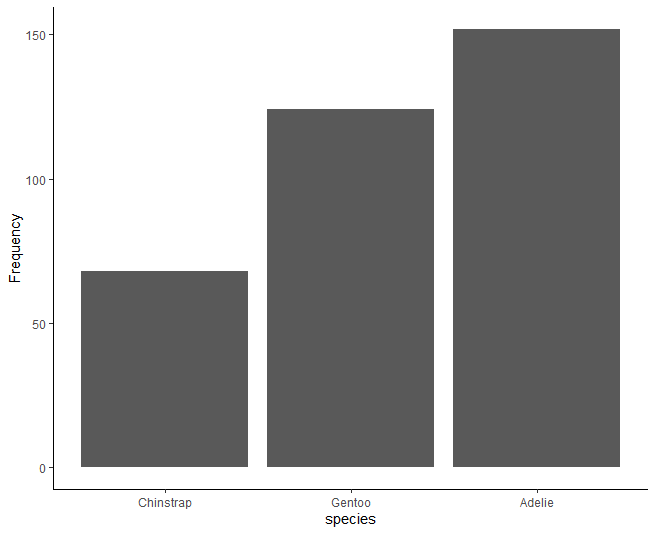
\includegraphics{images/frequency_bar.png}
\caption{Fig. 1: Species frequency in the penguins dataset.}
\end{figure}

It appears that Adelie pinguins are the most abundant in the dataset.
Now let's see if there are differences among islands:

Table 1: Individuals count per island that are part of the
``palmerpenguins'' package.

\begin{longtable}[]{@{}lrrrr@{}}
\toprule\noalign{}
island & Adelie & Chinstrap & Gentoo & Total \\
\midrule\noalign{}
\endhead
\bottomrule\noalign{}
\endlastfoot
Biscoe & 44 & 0 & 124 & 168 \\
Dream & 56 & 68 & 0 & 124 \\
Torgersen & 52 & 0 & 0 & 52 \\
Total & 152 & 68 & 124 & 344 \\
\end{longtable}

and in a graph:

\begin{figure}
\centering
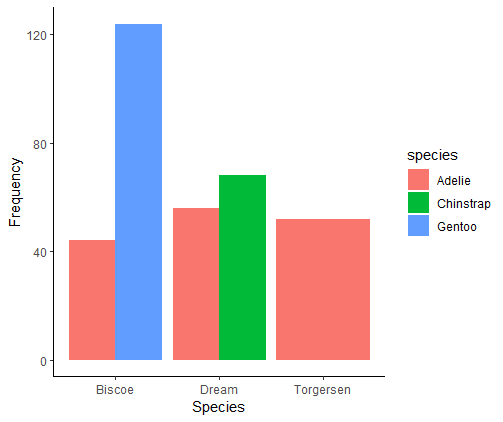
\includegraphics[width=5.29167in,height=\textheight]{images/island-penguin-02.png}
\caption{Fig. 2: Species distribution across islands in the
`palmerpenguins' package.}
\end{figure}

We did not violated any assumptions for the \(\chi^{2}\) test, so we can
say that the probability of being finding one penguin species is
significantly associated with the island where we are surveying
(\(\chi^{2}\) contingency test; \emph{df} = 4; \(\chi^{2}\) = 299.55;
\emph{P} \textless{} 0.001). Based on our bar plot (Fig. 2), the
distribution of penguins is vastly different among islands.

Cheers.

\hypertarget{discussion}{%
\subsubsection{Discussion}\label{discussion}}

We, indeed did found that penguin species is related to the island where
they are surveyed. Shocking. I do not know what else to say, mate.
\emph{Torgersen} are everywhere, and both \emph{Dream} and \emph{Biscoe}
are locked to particular islands. Neat.

\hypertarget{tables}{%
\subsubsection{Tables}\label{tables}}

Table 1: Individuals count per island that are part of the
``palmerpenguins'' package.

\begin{longtable}[]{@{}lrrrr@{}}
\toprule\noalign{}
island & Adelie & Chinstrap & Gentoo & Total \\
\midrule\noalign{}
\endhead
\bottomrule\noalign{}
\endlastfoot
Biscoe & 44 & 0 & 124 & 168 \\
Dream & 56 & 68 & 0 & 124 \\
Torgersen & 52 & 0 & 0 & 52 \\
Total & 152 & 68 & 124 & 344 \\
\end{longtable}

\hypertarget{figure-captions}{%
\subsubsection{Figure captions}\label{figure-captions}}

Fig. 1: Species frequency in the penguins dataset.

Fig. 2: Species distribution across islands in the `palmerpenguins'
package.

\hypertarget{figures}{%
\subsubsection{Figures}\label{figures}}

\begin{figure}
\centering
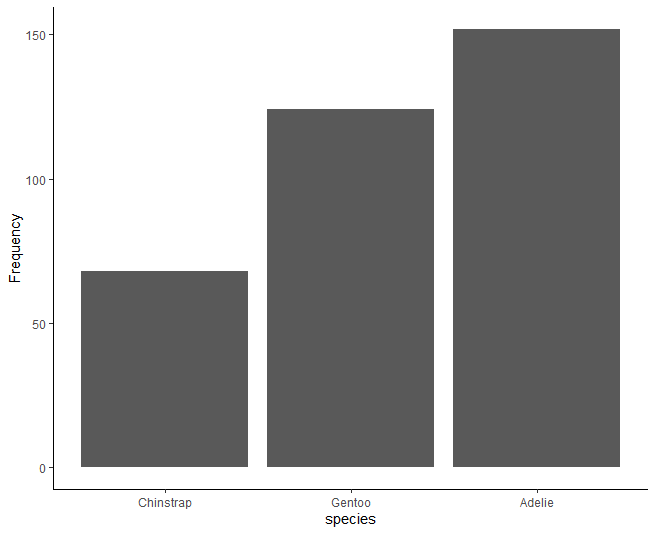
\includegraphics{images/frequency_bar.png}
\caption{Fig. 1: Species frequency in the penguins dataset.}
\end{figure}

\includegraphics{}

\hypertarget{appendices}{%
\subsubsection{Appendices}\label{appendices}}

See the PREE.R script for how this was done?

\hypertarget{references}{%
\subsubsection*{References}\label{references}}
\addcontentsline{toc}{subsubsection}{References}

\hypertarget{refs}{}
\begin{CSLReferences}{0}{0}
\leavevmode\vadjust pre{\hypertarget{ref-cahill2013}{}}%
Cahill, A.E., Aiello-Lammens, M.E., Fisher-Reid, M.C., Hua, X.,
Karanewsky, C.J., Yeong Ryu, H., \emph{et al.} (2013)
\href{https://doi.org/10.1098/rspb.2012.1890}{How does climate change
cause extinction?} \emph{Proceedings of the Royal Society B: Biological
Sciences}, \textbf{280}, 20121890.

\leavevmode\vadjust pre{\hypertarget{ref-carey2003}{}}%
Carey, C. \& Alexander, M.A. (2003)
\href{https://www.jstor.org/stable/3246804}{Climate change and amphibian
declines: Is there a link?} \emph{Diversity and Distributions},
\textbf{9}, 111--121.

\leavevmode\vadjust pre{\hypertarget{ref-harvey2023}{}}%
Harvey, J.A., Tougeron, K., Gols, R., Heinen, R., Abarca, M., Abram,
P.K., \emph{et al.} (2023)
\href{https://doi.org/10.1002/ecm.1553}{Scientists' warning on climate
change and insects}. \emph{Ecological Monographs}, \textbf{93}.

\end{CSLReferences}

\end{document}
